\section{Spark::Sp\-Tuple3$<$ Real $>$ Class Template Reference}
\label{classSpark_1_1SpTuple3}\index{Spark::SpTuple3@{Spark::SpTuple3}}
{\tt \#include $<$Sp\-Tuple.h$>$}

Inheritance diagram for Spark::Sp\-Tuple3$<$ Real $>$:\begin{figure}[H]
\begin{center}
\leavevmode
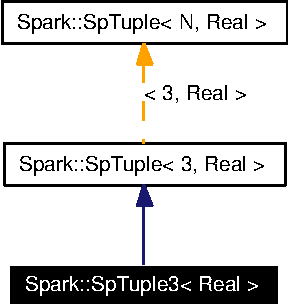
\includegraphics[width=86pt]{classSpark_1_1SpTuple3__inherit__graph}
\end{center}
\end{figure}
Collaboration diagram for Spark::Sp\-Tuple3$<$ Real $>$:\begin{figure}[H]
\begin{center}
\leavevmode
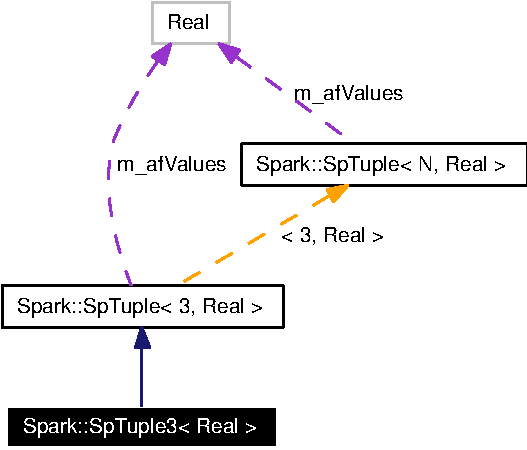
\includegraphics[width=144pt]{classSpark_1_1SpTuple3__coll__graph}
\end{center}
\end{figure}


\subsection{Detailed Description}
\subsubsection*{template$<$class Real$>$ class Spark::Sp\-Tuple3$<$ Real $>$}

3D tuple data class with support for vector mathematics 

Definition at line 141 of file Sp\-Tuple.h.\subsection*{Public Member Functions}
\begin{CompactItemize}
\item 
{\bf Sp\-Tuple3} (const {\bf Sp\-Tuple}$<$ 3, Real $>$ \&rk\-V)
\begin{CompactList}\small\item\em Construction. \item\end{CompactList}\item 
{\bf Sp\-Tuple3} (Real f\-X=0, Real f\-Y=0, Real f\-Z=0)
\item 
Real {\bf x} () const
\begin{CompactList}\small\item\em Position Coordinate Access:. \item\end{CompactList}\item 
Real \& {\bf x} ()
\item 
Real {\bf y} () const
\item 
Real \& {\bf y} ()
\item 
Real {\bf z} () const
\item 
Real \& {\bf z} ()
\item 
Real {\bf r} () const
\begin{CompactList}\small\item\em Color Component Access:. \item\end{CompactList}\item 
Real \& {\bf r} ()
\item 
Real {\bf g} () const
\item 
Real \& {\bf g} ()
\item 
Real {\bf b} () const
\item 
Real \& {\bf b} ()
\item 
Real {\bf s} () const
\begin{CompactList}\small\item\em Texture Coordinate Access:. \item\end{CompactList}\item 
Real \& {\bf s} ()
\item 
Real {\bf t} () const
\item 
Real \& {\bf t} ()
\item 
Real {\bf p} () const
\item 
Real \& {\bf p} ()
\end{CompactItemize}


\subsection{Constructor \& Destructor Documentation}
\index{Spark::SpTuple3@{Spark::Sp\-Tuple3}!SpTuple3@{SpTuple3}}
\index{SpTuple3@{SpTuple3}!Spark::SpTuple3@{Spark::Sp\-Tuple3}}
\subsubsection{\setlength{\rightskip}{0pt plus 5cm}template$<$class Real$>$ {\bf Spark::Sp\-Tuple3}$<$ Real $>$::{\bf Sp\-Tuple3} (const {\bf Sp\-Tuple}$<$ 3, Real $>$ \& {\em rk\-V})\hspace{0.3cm}{\tt  [inline]}}\label{classSpark_1_1SpTuple3_a0}


Construction. 

Definition at line 147 of file Sp\-Tuple.h.\index{Spark::SpTuple3@{Spark::Sp\-Tuple3}!SpTuple3@{SpTuple3}}
\index{SpTuple3@{SpTuple3}!Spark::SpTuple3@{Spark::Sp\-Tuple3}}
\subsubsection{\setlength{\rightskip}{0pt plus 5cm}template$<$class Real$>$ {\bf Spark::Sp\-Tuple3}$<$ Real $>$::{\bf Sp\-Tuple3} (Real {\em f\-X} = {\tt 0}, Real {\em f\-Y} = {\tt 0}, Real {\em f\-Z} = {\tt 0})\hspace{0.3cm}{\tt  [inline]}}\label{classSpark_1_1SpTuple3_a1}


Definition at line 150 of file Sp\-Tuple.h.

References Spark::Sp\-Tuple3$<$ Real $>$::x(), Spark::Sp\-Tuple3$<$ Real $>$::y(), and Spark::Sp\-Tuple3$<$ Real $>$::z().

\subsection{Member Function Documentation}
\index{Spark::SpTuple3@{Spark::Sp\-Tuple3}!b@{b}}
\index{b@{b}!Spark::SpTuple3@{Spark::Sp\-Tuple3}}
\subsubsection{\setlength{\rightskip}{0pt plus 5cm}template$<$class Real$>$ Real\& {\bf Spark::Sp\-Tuple3}$<$ Real $>$::b ()\hspace{0.3cm}{\tt  [inline]}}\label{classSpark_1_1SpTuple3_a13}


Definition at line 171 of file Sp\-Tuple.h.\index{Spark::SpTuple3@{Spark::Sp\-Tuple3}!b@{b}}
\index{b@{b}!Spark::SpTuple3@{Spark::Sp\-Tuple3}}
\subsubsection{\setlength{\rightskip}{0pt plus 5cm}template$<$class Real$>$ Real {\bf Spark::Sp\-Tuple3}$<$ Real $>$::b () const\hspace{0.3cm}{\tt  [inline]}}\label{classSpark_1_1SpTuple3_a12}


Definition at line 170 of file Sp\-Tuple.h.\index{Spark::SpTuple3@{Spark::Sp\-Tuple3}!g@{g}}
\index{g@{g}!Spark::SpTuple3@{Spark::Sp\-Tuple3}}
\subsubsection{\setlength{\rightskip}{0pt plus 5cm}template$<$class Real$>$ Real\& {\bf Spark::Sp\-Tuple3}$<$ Real $>$::g ()\hspace{0.3cm}{\tt  [inline]}}\label{classSpark_1_1SpTuple3_a11}


Definition at line 169 of file Sp\-Tuple.h.\index{Spark::SpTuple3@{Spark::Sp\-Tuple3}!g@{g}}
\index{g@{g}!Spark::SpTuple3@{Spark::Sp\-Tuple3}}
\subsubsection{\setlength{\rightskip}{0pt plus 5cm}template$<$class Real$>$ Real {\bf Spark::Sp\-Tuple3}$<$ Real $>$::g () const\hspace{0.3cm}{\tt  [inline]}}\label{classSpark_1_1SpTuple3_a10}


Definition at line 168 of file Sp\-Tuple.h.\index{Spark::SpTuple3@{Spark::Sp\-Tuple3}!p@{p}}
\index{p@{p}!Spark::SpTuple3@{Spark::Sp\-Tuple3}}
\subsubsection{\setlength{\rightskip}{0pt plus 5cm}template$<$class Real$>$ Real\& {\bf Spark::Sp\-Tuple3}$<$ Real $>$::p ()\hspace{0.3cm}{\tt  [inline]}}\label{classSpark_1_1SpTuple3_a19}


Definition at line 181 of file Sp\-Tuple.h.\index{Spark::SpTuple3@{Spark::Sp\-Tuple3}!p@{p}}
\index{p@{p}!Spark::SpTuple3@{Spark::Sp\-Tuple3}}
\subsubsection{\setlength{\rightskip}{0pt plus 5cm}template$<$class Real$>$ Real {\bf Spark::Sp\-Tuple3}$<$ Real $>$::p () const\hspace{0.3cm}{\tt  [inline]}}\label{classSpark_1_1SpTuple3_a18}


Definition at line 180 of file Sp\-Tuple.h.\index{Spark::SpTuple3@{Spark::Sp\-Tuple3}!r@{r}}
\index{r@{r}!Spark::SpTuple3@{Spark::Sp\-Tuple3}}
\subsubsection{\setlength{\rightskip}{0pt plus 5cm}template$<$class Real$>$ Real\& {\bf Spark::Sp\-Tuple3}$<$ Real $>$::r ()\hspace{0.3cm}{\tt  [inline]}}\label{classSpark_1_1SpTuple3_a9}


Definition at line 167 of file Sp\-Tuple.h.\index{Spark::SpTuple3@{Spark::Sp\-Tuple3}!r@{r}}
\index{r@{r}!Spark::SpTuple3@{Spark::Sp\-Tuple3}}
\subsubsection{\setlength{\rightskip}{0pt plus 5cm}template$<$class Real$>$ Real {\bf Spark::Sp\-Tuple3}$<$ Real $>$::r () const\hspace{0.3cm}{\tt  [inline]}}\label{classSpark_1_1SpTuple3_a8}


Color Component Access:. 

Definition at line 166 of file Sp\-Tuple.h.\index{Spark::SpTuple3@{Spark::Sp\-Tuple3}!s@{s}}
\index{s@{s}!Spark::SpTuple3@{Spark::Sp\-Tuple3}}
\subsubsection{\setlength{\rightskip}{0pt plus 5cm}template$<$class Real$>$ Real\& {\bf Spark::Sp\-Tuple3}$<$ Real $>$::s ()\hspace{0.3cm}{\tt  [inline]}}\label{classSpark_1_1SpTuple3_a15}


Definition at line 177 of file Sp\-Tuple.h.\index{Spark::SpTuple3@{Spark::Sp\-Tuple3}!s@{s}}
\index{s@{s}!Spark::SpTuple3@{Spark::Sp\-Tuple3}}
\subsubsection{\setlength{\rightskip}{0pt plus 5cm}template$<$class Real$>$ Real {\bf Spark::Sp\-Tuple3}$<$ Real $>$::s () const\hspace{0.3cm}{\tt  [inline]}}\label{classSpark_1_1SpTuple3_a14}


Texture Coordinate Access:. 

Definition at line 176 of file Sp\-Tuple.h.\index{Spark::SpTuple3@{Spark::Sp\-Tuple3}!t@{t}}
\index{t@{t}!Spark::SpTuple3@{Spark::Sp\-Tuple3}}
\subsubsection{\setlength{\rightskip}{0pt plus 5cm}template$<$class Real$>$ Real\& {\bf Spark::Sp\-Tuple3}$<$ Real $>$::t ()\hspace{0.3cm}{\tt  [inline]}}\label{classSpark_1_1SpTuple3_a17}


Definition at line 179 of file Sp\-Tuple.h.\index{Spark::SpTuple3@{Spark::Sp\-Tuple3}!t@{t}}
\index{t@{t}!Spark::SpTuple3@{Spark::Sp\-Tuple3}}
\subsubsection{\setlength{\rightskip}{0pt plus 5cm}template$<$class Real$>$ Real {\bf Spark::Sp\-Tuple3}$<$ Real $>$::t () const\hspace{0.3cm}{\tt  [inline]}}\label{classSpark_1_1SpTuple3_a16}


Definition at line 178 of file Sp\-Tuple.h.\index{Spark::SpTuple3@{Spark::Sp\-Tuple3}!x@{x}}
\index{x@{x}!Spark::SpTuple3@{Spark::Sp\-Tuple3}}
\subsubsection{\setlength{\rightskip}{0pt plus 5cm}template$<$class Real$>$ Real\& {\bf Spark::Sp\-Tuple3}$<$ Real $>$::x ()\hspace{0.3cm}{\tt  [inline]}}\label{classSpark_1_1SpTuple3_a3}


Definition at line 157 of file Sp\-Tuple.h.\index{Spark::SpTuple3@{Spark::Sp\-Tuple3}!x@{x}}
\index{x@{x}!Spark::SpTuple3@{Spark::Sp\-Tuple3}}
\subsubsection{\setlength{\rightskip}{0pt plus 5cm}template$<$class Real$>$ Real {\bf Spark::Sp\-Tuple3}$<$ Real $>$::x () const\hspace{0.3cm}{\tt  [inline]}}\label{classSpark_1_1SpTuple3_a2}


Position Coordinate Access:. 

Definition at line 156 of file Sp\-Tuple.h.

Referenced by Spark::Sp\-Tuple3$<$ Real $>$::Sp\-Tuple3().\index{Spark::SpTuple3@{Spark::Sp\-Tuple3}!y@{y}}
\index{y@{y}!Spark::SpTuple3@{Spark::Sp\-Tuple3}}
\subsubsection{\setlength{\rightskip}{0pt plus 5cm}template$<$class Real$>$ Real\& {\bf Spark::Sp\-Tuple3}$<$ Real $>$::y ()\hspace{0.3cm}{\tt  [inline]}}\label{classSpark_1_1SpTuple3_a5}


Definition at line 159 of file Sp\-Tuple.h.\index{Spark::SpTuple3@{Spark::Sp\-Tuple3}!y@{y}}
\index{y@{y}!Spark::SpTuple3@{Spark::Sp\-Tuple3}}
\subsubsection{\setlength{\rightskip}{0pt plus 5cm}template$<$class Real$>$ Real {\bf Spark::Sp\-Tuple3}$<$ Real $>$::y () const\hspace{0.3cm}{\tt  [inline]}}\label{classSpark_1_1SpTuple3_a4}


Definition at line 158 of file Sp\-Tuple.h.

Referenced by Spark::Sp\-Tuple3$<$ Real $>$::Sp\-Tuple3().\index{Spark::SpTuple3@{Spark::Sp\-Tuple3}!z@{z}}
\index{z@{z}!Spark::SpTuple3@{Spark::Sp\-Tuple3}}
\subsubsection{\setlength{\rightskip}{0pt plus 5cm}template$<$class Real$>$ Real\& {\bf Spark::Sp\-Tuple3}$<$ Real $>$::z ()\hspace{0.3cm}{\tt  [inline]}}\label{classSpark_1_1SpTuple3_a7}


Definition at line 161 of file Sp\-Tuple.h.\index{Spark::SpTuple3@{Spark::Sp\-Tuple3}!z@{z}}
\index{z@{z}!Spark::SpTuple3@{Spark::Sp\-Tuple3}}
\subsubsection{\setlength{\rightskip}{0pt plus 5cm}template$<$class Real$>$ Real {\bf Spark::Sp\-Tuple3}$<$ Real $>$::z () const\hspace{0.3cm}{\tt  [inline]}}\label{classSpark_1_1SpTuple3_a6}


Definition at line 160 of file Sp\-Tuple.h.

Referenced by Spark::Sp\-Tuple3$<$ Real $>$::Sp\-Tuple3().

The documentation for this class was generated from the following file:\begin{CompactItemize}
\item 
{\bf Sp\-Tuple.h}\end{CompactItemize}
